\documentclass{article}

\usepackage[utf8]{inputenc}
\usepackage[T1]{fontenc}
\usepackage[frenchb]{babel}
\usepackage{amsmath,amsfonts,amssymb,amsthm}
\usepackage[margin=1in]{geometry}
\usepackage{graphicx}
\usepackage{hyperref}

\setcounter{secnumdepth}{0}
\graphicspath{ {./Images/} }

\begin{document}

\begin{titlepage}

	\begin{center}
		\hrule

		\vspace{.5cm}

		\Huge
		\textbf{Téléinformatique}

		\vspace{.3cm}
		\LARGE

		\textbf{IFT 3325}
		\vspace{.3cm}

		\textbf{Devoir n°3}
		\vspace{.3cm}

		\hrule

		\vspace{1cm}

		17 Décembre 2023 \\
	\end{center}

	\vspace{2cm}

	\LARGE

	\noindent Auteurs :

	\begin{enumerate}
		\item[-] Léo Jetzer (20070432)
		\item[-] Luchino Allix-Lastrego (20222844)   
	\end{enumerate}


			
	\vfill


	\begin{center}

		%
\includegraphics[scale=.1]{diro.png}

		\vspace{0.8cm}

		Université de Montréal\\
		Département d'informatique et de recherche opérationnelle\\

	\end{center}
	
\end{titlepage}

\section{Exercice 1 \emph{(10 points)}}

\subsection{a. \emph{(6 points)}} % A developper

Pour réduire la charge d'un serveur il faut favoriser l'utilisation de Go-Back-N car les acknowledge cumulatifs permettent de diminuer le nombre de réponses par rapport au grand nombre de petits messages.

\subsection{b. \emph{(4 points)}}
S'il y a une erreur lors de la lecture d'une trame et qu'elle est rejetée, il est posssible que le fanion qui était supposé marquer la fin soit interprété comme le début d'une nouvelle trame. On essai alors de lire des trames qui n'existe pas et/ou d'ignorer les vrais trames.

\clearpage

\section{Exercice 2 \emph{(16 points)}}

\subsection{Dijkstra}

Dans le tableau ci-dessous, les colonnes indiquent les sommets et les lignes le sommet où l'on est actuellement. Par exemple \emph{E (5)} signifie qu'on se trouve sur le sommet E et que le poid associé pour arriver à ce sommet est de 5. Le croisement entre une ligne et une colonne indique comment faire pour arriver à ce sommet. Par exemple, \emph{5 B} à la ligne \emph{H (4)} et à la colonne \emph{C} indique que pour se rendre en \emph{C} le plus court chemin vaut 5 et passe par \emph{B}. Le symbole $\infty$ indique que le sommet n'a pas encore pu être atteint et '-' indique que le chemin à déjà été visité. 

\hfill

\begin{tabular}{|c|c|c|c|c|c|c|c|c|c|c|c|}
	\hline
	& A & B & C & D & E & F & G & H & I & J & Z\\
	\hline
	Départ & 0 A & $\infty$ & $\infty$ & $\infty$ & $\infty$ & $\infty$ & $\infty$ & $\infty$ & $\infty$ & $\infty$ & $\infty$\\
	\hline 
	A (0) & - & 3 A & $\infty$ & $\infty$ & 5 A & $\infty$ & $\infty$ & 4 A & $\infty$ & $\infty$ & $\infty$\\
	\hline
	B (3) & - & - & 5 B & $\infty$ & 5 A & 10 B & $\infty$ & 4 A & $\infty$ & $\infty$ & $\infty$\\
	\hline
	H (4) & - & - & 5 B & $\infty$ & 5 A & 9 H & $\infty$ & - & 6 H & $\infty$ & $\infty$\\
	\hline
	E (5) & - & - & 5 B & $\infty$ & - & 9 H & $\infty$ & - & 6 H & $\infty$ & $\infty$\\
	\hline
	C (5) & - & - & - & 8 C & - & 7 C & 11 C & - & 6 H & $\infty$ & $\infty$\\
	\hline
	I (6) & - & - & - & 8 C & - & 7 C & 11 C & - & - & 12 I & $\infty$\\
	\hline
	F (7) & - & - & - & 8 C & - & - & 11 C & - & - & 10 F & $\infty$\\
	\hline
	D (8) & - & - & - & - & - & - & 11 C & - & - & 10 F & 10 D\\
	\hline
\end{tabular}

\hfill

\hfill

À la dernière ligne du tableau, on voit que l'on peut arriver en \emph{Z} en venant de D avec un chemin de poid 10. Ceci met fin à l'algorithme car les autres chemins qui n'arrivent pas encore à \emph{Z} sont de poid supérieur ou égal à 10. Pour retrouver le chemin parcouru on remonte le tableau. On arrive en \emph{Z} depuis \emph{D}, on arrive en \emph{D} depuis \emph{C} et ainsi de suite pour obtenir le chemin  de poid 10 : \emph{ABCDZ}.

\subsection{Bellman-Ford}

Dans le tableau ci dessous, les colonnes indiquent le sommet et les lignes le nombre maximum de chemin que l'on peut prendre pour arriver au sommet. La logique reste la même concerant les cases. Par exemple \emph{5 B} à la ligne \emph{4} et à la colonne \emph{C} indique que pour se rendre en \emph{C} avec au plus 4 chemins emprunté, le plus court chemin vaut 5 et passe par \emph{B}.Comme précedement $\infty$ indique que le sommet n'a pas encore pu être atteint.

\hfill

\begin{tabular}{|c|c|c|c|c|c|c|c|c|c|c|c|}
	\hline
	Itération & A & B & C & D & E & F & G & H & I & J & Z\\
	\hline
	0 & 0 A & $\infty$ & $\infty$ & $\infty$ & $\infty$ & $\infty$ & $\infty$ & $\infty$ & $\infty$ & $\infty$ & $\infty$\\
	\hline 
	1 & 0 A & 3 A & $\infty$ & $\infty$ & 5 A & $\infty$ & $\infty$ & 4 A & $\infty$ & $\infty$ & $\infty$\\
	\hline
	2 & 0 A & 3 A & 5 B & $\infty$ & 5 A & 9 E & $\infty$ & 4 A & 6 H & $\infty$ & $\infty$\\
	\hline
	3 & 0 A & 3 A & 5 B & 8 C & 5 A & 7 C & 11 C & 4 A & 6 H & 12 I & $\infty$\\
	\hline
	4 & 0 A & 3 A & 5 B & 8 C & 5 A & 7 C & 11 C & 4 A & 6 H & 10 F & 10 D\\
	\hline
	5 & 0 A & 3 A & 5 B & 8 C & 5 A & 7 C & 11 C & 4 A & 6 H & 10 F & 10 D\\
	\hline
	6 & 0 A & 3 A & 5 B & 8 C & 5 A & 7 C & 11 C & 4 A & 6 H & 10 F & 10 D\\
	\hline
	7 & 0 A & 3 A & 5 B & 8 C & 5 A & 7 C & 11 C & 4 A & 6 H & 10 F & 10 D\\
	\hline
	8 & 0 A & 3 A & 5 B & 8 C & 5 A & 7 C & 11 C & 4 A & 6 H & 10 F & 10 D\\
	\hline
	9 & 0 A & 3 A & 5 B & 8 C & 5 A & 7 C & 11 C & 4 A & 6 H & 10 F & 10 D\\
	\hline
	10 & 0 A & 3 A & 5 B & 8 C & 5 A & 7 C & 11 C & 4 A & 6 H & 10 F & 10 D\\
	\hline
\end{tabular}

\hfill

\hfill

On remarque que à partir de la ligne 4, plus rien ne change, en effet tous les plus courts chemins depuis le sommet A vers les autres sommets empruntent au plus 4 arrêtes. Pour trouver le chemin le plus court de \emph{A} à \emph{Z} même logique que précedement, ce qui nous donne : \emph{ABCDZ} avec un poid de 10.


\clearpage

\section{Exercice 3 \emph{(12 points)}}

\subsection{a. \emph{(6 points)}} % A developper 

On remarque que :


\noindent \begin{minipage}{9cm}
	\begin{align*}
		A &= 01100101.01000000.00000000.01100110\\
		M &= 11111111.11111111.00000000.00000000\\
		A \land  M &= 01100101.01000000.00000000.00000000\\
	\end{align*}
\end{minipage}
\begin{minipage}{7cm}
	\begin{align*}
		B &= 01100101.01000000.00101101.01100110\\
		M &= 11111111.11111111.00000000.00000000\\
		B \land  M &= 01100101.01000000.00000000.00000000\\
	\end{align*}
\end{minipage}

\hfill

Ce qui veut dire que $A$  et $B$ ont le même réseau, or avec ce masque, il n'y a qu'un seul sous réseau disponible. En effet, vu que $A \land  M = B \land  M$ ils appartiennent donc au même sous réseau. Donc TCP/IP n'est pas le bon médium de communication. 

\subsection{b. \emph{(6 points)}}

Oui il faut modifier cette table de routage car pour se rendre en D, la table indique que la passerelle est 192.168.51.1 alors qu'elle devrait être 192.168.52.2.

\clearpage

\section{Exercice 4 \emph{(10 points)}}

\subsection{a. \emph{(3 points)}}

Lors de l'établissement d'une connexion au niveau de la couche transport, on peut négocier :

\begin{enumerate}
	\item La taille maximale de la fenêtre. Pour améliorer l'efficacité.
	\item La taille maximale de segment. Pour permettre de lire correctement les paquets.
	\item L'utilisation du timestamps. Ceci permet de faciliter l'ordre dans lequel les paquets ont été envoyé. 
\end{enumerate}

\subsection{b. \emph{(4 points)}}
\begin{itemize}
    \item \textbf{Length}: Change de la taille total du paquet à la taille du fragment
    \item \textbf{fragFlag}/\textbf{bit More}: Indique s'il s'agit du dernier fragment
    \item \textbf{Offset}: offset du premier bit pertinent du fragment relatif au début du paquet
\end{itemize}
Bien entendu, les donnés contenues changes aussi.

\subsection{c. \emph{(3 points)}}
\begin{itemize}
    \item Le routeur doit ré-assembler/désassembler chaque paquet qu'il reçoit et transmet, consommant beaucoup de ressources. Un paquet peut donc être ré-assembler/désassembler plusieurs fois lors de sa transmission. Par contre, la quantité de paquet circulant est optimisée
    \item Chaque paquet est ré-assembler/désassembler une seule fois, à la source et la destination. Il faut par contre connaître d'avance la plus petite taille de paquet autorisée sur le chemin.
\end{itemize}

\clearpage

\section{Exercice 5 \emph{(12 points)}}
%Un deadlock se produit si au moins une des machines attend une réponse spécifique avant de procéder d'avantage et que l'autre machine fait tout sauf l'envoyer (généralement parce qu'elle attend elle aussi une réponse avant de procéder). 

%Les two-way handshake ont des problèmes, mais les deadlocks n'en sont généralement pas un. Par contre, si une des machines pense qu'il s'agit d'un three-way handshake et attend le deuxième \verb|ACK| avant de procéder, elle va attendre longtemps.

%Ex:
%\begin{enumerate}
%    \item A envoi un \verb|SYN| à B
%    \item B reçoit le \verb|SYN| et envoi un \verb|ACK|
%    \item A reçoit le \verb|ACK|. Puisque A utilisait un two-way handshake, il trouve que c'est suffisant et envoi ses données.
%    \item B s'attend à recevoir un autre \verb|ACK| et ignore toutes les données.
%\end{enumerate}
%Puisque les réponses pour des two-way et three-way handshake sont différentes, il est possible de s'adpater aux réponses reçu et d'éviter les deadlocks.

Les deadlocks n'étaient pas le problème principale des two-way handshake, mais ils arrivaient quand même.

Voici un deadlock possible :
\begin{enumerate}
    \item A envoi SYN
    \item B reçoit SYN et envoi un SYN en retour
    \item ce dernier et perdu, donc A ne le reçoit pas
    \item le temporisateur de A expire sans qu'il aie reçu une réponse, alors il renvoi un SYN
    \item B reçoit ce SYN, mais comme la connexion est déjà ouverte, il l'ignore et attend les données
    \item A n'a toujours pas de réponse et continue d'envoyer des SYN et B continue de les ignorer
\end{enumerate}

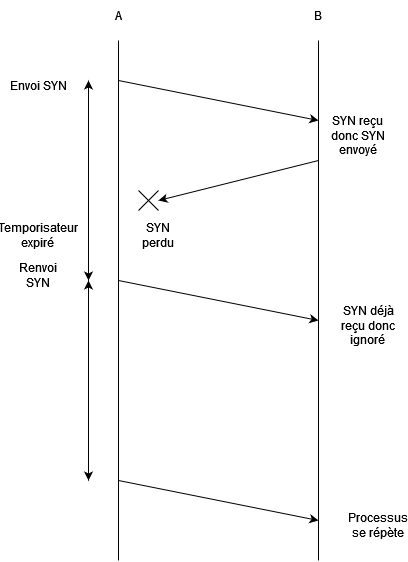
\includegraphics[scale=1]{q5.png}


\clearpage

\section{Exercice 6 \emph{(12 points)}}
J'ai de la difficulté à comprendre la question, alors voici des solutions selon différentes manière de l'interpréter

\begin{align*}
    T &: \text{threshold de la taille de la fenêtre avant de ralentir l'agrandissement} \\
    n &: \text{nombre de segment à envoyer.} = \left\lceil \frac{M}{N} \right\rceil \\
    F &: \text{Taille maximale de la fenêtre} \\
    t &: \text{nb de RT nécessaire pour que la fenêtre atteigne la taille $T$.} = \left\lceil\lg(T+1)\right\rceil \\
    q(i) &: \text{nb de segments envoyés au RT $i$.} = 
    \left\{\begin{array}{ll}
         0 & \text{si } i\leq 0 \\
         2^{i-1} & \text{si } 0 < i \leq t \\
         \min(F, 2^{t-1}+i-t) & \text{sinon}
    \end{array}\right.\\
    Q(i) &: \text{nb total de segments envoyés après un RTT $i$.} = \displaystyle\sum_{j=0}^{i} q(j)
\end{align*}

\subsection{Envoyer M octets en 1 RT}
On veut simplement trouver un $i$ tq. $q(i-1) < n \leq q(i)$

Si $n \leq T$ alors la quantité de RT nécessaire pour envoyer $M$ octets en un RT est $\left\lceil\lg{n}\right\rceil+1$.
Sinon, elle est de $\left\lceil\lg{T}\right\rceil + 1 + n - T$

\subsection{Envoyer M octets en tout}
Pour $n$ segments, on veut donc trouver un $i$ tq. $Q(i-1) < m \leq Q(i)$.

Si $n \leq Q(t)$ (ie. $i \leq t$), alors $Q(i) = 2^i - 1$ donc $i = \left\lceil\lg(n+1)\right\rceil$

\hfill

-------------------------- Ma version ----------------------

\hfill

On doit transmettre $M$ octets au nième aller retour, or la taille d'un segment est de $N$ octets. Donc avec un slow start on commence avec $N$ octets puis $2N$ puis $4N$ et ainsi de suite jusqu'à $2^{n-1}N$ octets (on veut commencer à $2^0$ avec n = 1 et non n = 0 car on aura alors fait 1 aller retour).

\hfill

On veut envoyer au moins $M$ octets donc il faut que 

$$ 2^{n-1} N \geqslant M  $$ donc $$ 2^{n-1} \geqslant \frac{M}{N} $$ donc $$ n \geqslant \log_2\left(\frac{M}{N}\right)$$
On en conclu que $$ n = \left\lceil \log_2\left(\frac{M}{N}\right)\right\rceil +1$$

\clearpage

\section{Exercice 7 \emph{(7 points)}}

Non les réseaux à circuits virtuel n'ont pas besoin d'être capable de router des paquets isolé car ils suivent tous un chemin prédéfini. Si on parle d'un paquet qui possède sa destination (qui a été poussé dans le canal quand la connexion à été établie) et qu'il fait parti du circuit virtuel alors aucun routage n'est necessaire, il est dans le circuit et il n'a qu'à le suivre.


\section{Exercice 8 \emph{(10 points)}}
La durée d'un RT est de $1 + 3 + 2 + 1 + 3 = 10$ unités. Si on assume qu'il n'y a aucune congestion et que la fenêtre de réception reste de la même taille constamment, il y a $7$ segments d'informations transmis chaque 10 unités au maximum.


\section{Exercice 9 \emph{(6 points)}}
Avec  une connection de 100Mbps et un RTT de 1ms, jusqu'à 125 bytes sont transféré à chaque RT.
Pour assurer un flux continue, il nous faut donc une fenêtre d'au moins 125 bytes (ça rentre bien dans un seul segment)


\section{Exercice 10 \emph{(5 points)}}

Non les algorithmes de Dijkstra et Bellman-Frod ne produisent pas tout le temps les mêmes résultats car l'algorithme de Dijkstra ne permet pas des arrêtes avec des poids négatifs alors que celui de Bellman-Ford oui. Donc dans un graph avec au moins une arrête de poid négatif, les deux algorithmes ne produiront pas peut être pas le même résultat.


\end{document}
